\subsection{ABAQUS Finite Element Analysis}

To provide accessible simulations of AFM imaging, our implementation of ABAQUS utilised Python scripts to produce simulations (see Appendix \ref{Appendix: ABAQUS Script}). An ABAQUS model defines seven basic modules (shown in Figure \ref{fig: ABAQUS Modules}): parts, properties, assembly, interactions, steps, loads/boundary conditions, and mesh. These moduli are defined within the Python code using predefined variables for the simulations, with geometric dimensions defined in nm and forces as pN. From this, a Python submission script is created and run by ABAQUS software. A brief outline of ABAQUS modelling follows.

\begin{figure}[H]
    \centering
    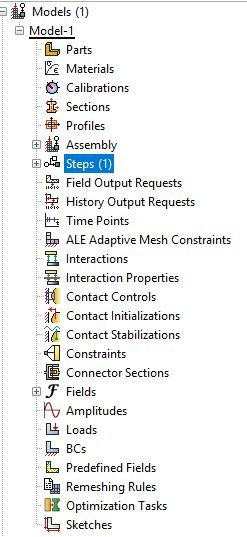
\includegraphics[width=0.32\linewidth]{Figures/Abaqus Modules.jpg}
    \caption{Display of model modules within ABAQUS GUI}
    \label{fig: ABAQUS Modules}
\end{figure}

The geometry of our simulation is the foundation of a model and is built as parts in the Parts module. Parts are formed from two-dimensional sketches that form a features profile. These profiles can be extruded, revolved, or swept to create part geometry or used directly to form a planar or axisymmetric part. Parts can be deformable, discrete rigid, analytical rigid, or Eulerian. The material properties and distribution for individual parts or sections of parts are set using the Properties module. The individual parts can then be joined and arranged in the Assembly module to create an assembly instance of the parts (known as part instances). 

The behaviour of the part instances are defined in the interaction module, and various loads and boundary conditions can be applied to the part instances within the Load module. The Mesh module then allows the geometry to be coarse-grained and the surface subdivided into small, discrete finite elements. The steps module defines the sequence of one or more analysis steps and the increments of the analysis at which dynamics are propagated. The steps track the changes in the loading and boundary conditions of the model. The model can then be submitted, and the ABAQUS software runs the Finite Element Analysis.

